\documentclass[preprint,10pt]{elsarticle}

\usepackage{amssymb}
\usepackage{amsmath}
\usepackage{lineno}
\usepackage{hyperref}

\usepackage{epstopdf}
\usepackage{epsfig}
\usepackage{setspace}

\newcommand{\be}{\begin{equation}}
\newcommand{\ee}{\end{equation}}
\newcommand{\beq}{\begin{eqnarray}}
\newcommand{\eeq}{\end{eqnarray}}
\newcommand{\ba}{\begin{eqnarray}}
\newcommand{\ea}{\end{eqnarray}}

\newcommand{\ua}{{\bf u}_\alpha}
\newcommand{\utwo}{\overline{\bf u}_2}
\setcounter{MaxMatrixCols}{24}

\journal{Coastal Engineering}

\begin{document}


%\title{Model derivations}

\begin{center}
{\bf \Huge Time-dependent wavemaker}
 \end{center}
 
 \section{Summary}
 
 1) The problem was caused by the wave-coherence which occurs as  phases for specified wave components are the same. The finding shows an extreme case with 100\% wave-coherence. 
 
 2) I used a simple MATLAB program to identify the problem. See the matlab scripts in the package, /Linear\_Program/
 
 3) In the modified Funwave code, I added a random function to generate random phases if a user does not specify phases in the input files. I also implemented an option that allows a user to output the linear theoretical solution for comparison with the numerical solution.  
 
 4) The time-dependent spectral wavemaker is documented in details. Hope it can help with further documentation/reports. 
 
 \section{The problem  } 
  
  Figure \ref{spec} shows the spectral distribution from your file: spectral\_data\_1.txt. I assume that the data is wave amplitude for each $\delta f \delta d$ cell and has a unit of meter. The significant wave height is 0.3704.  The matlab program for this plot can be found /Linear\_Program/mk\_spec\_brocc.m. 
  
The problem was found that, when you directly use the spectral files, the wave surface calculated from the model shows an inhomogeneous distribution of wave height, as shown in Figure \ref{tmp}. This inhomogeneous distribution is not due to any bugs in the code. It results from strong wave coherence, which occurs because the wave phases are the same at the wavemaker. Figure \ref{theoretical} shows the theoretical solution of the wave surface using the spectral file. It has the same pattern as the numerical solution. The theoretical solution will be described later in this document.
  
 \begin{figure}
\begin{center}
 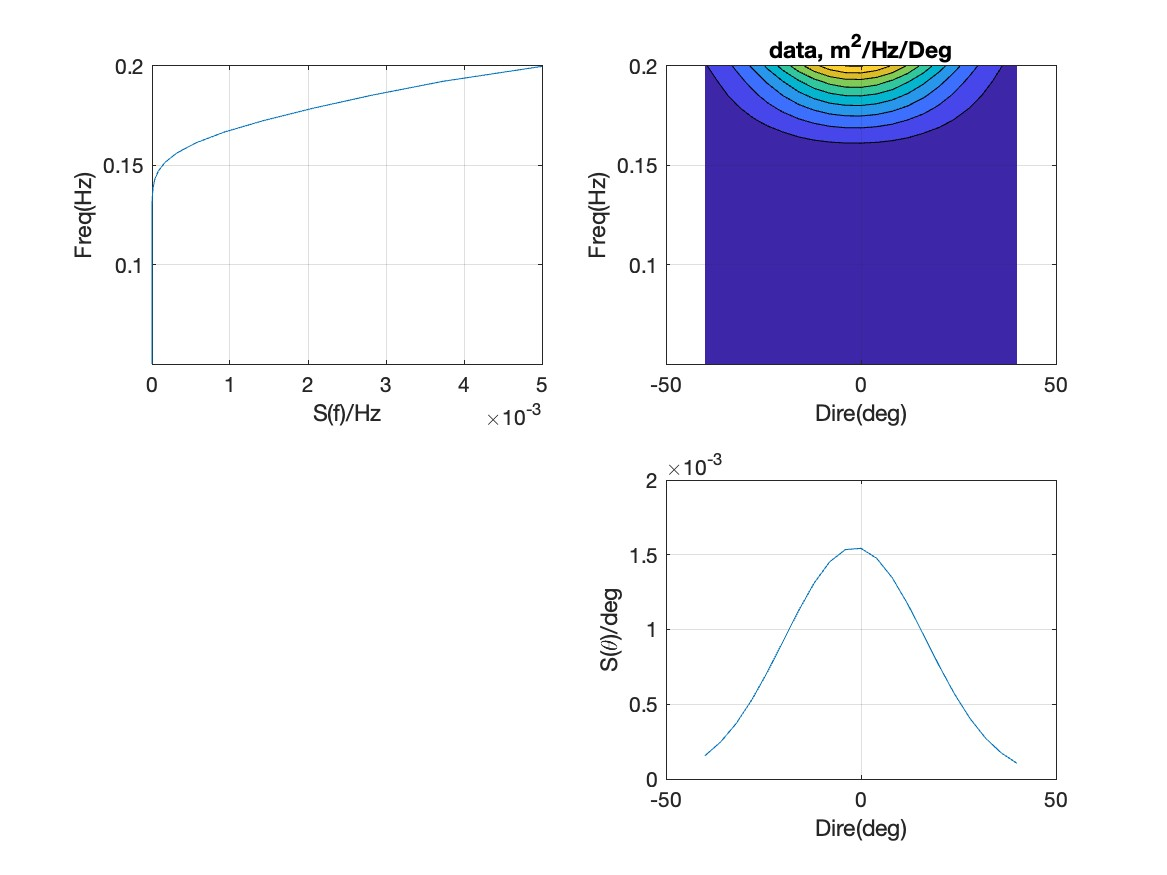
\includegraphics[width=1.0\textwidth]{figures/spectral.jpg}
 \caption{Spectral distribution from spectra\_data\_1.txt.  Use mk\_spec\_brocc.m. }
 \label{spec}
 \end{center}
 \end{figure}
  
  \begin{figure}
\begin{center}
 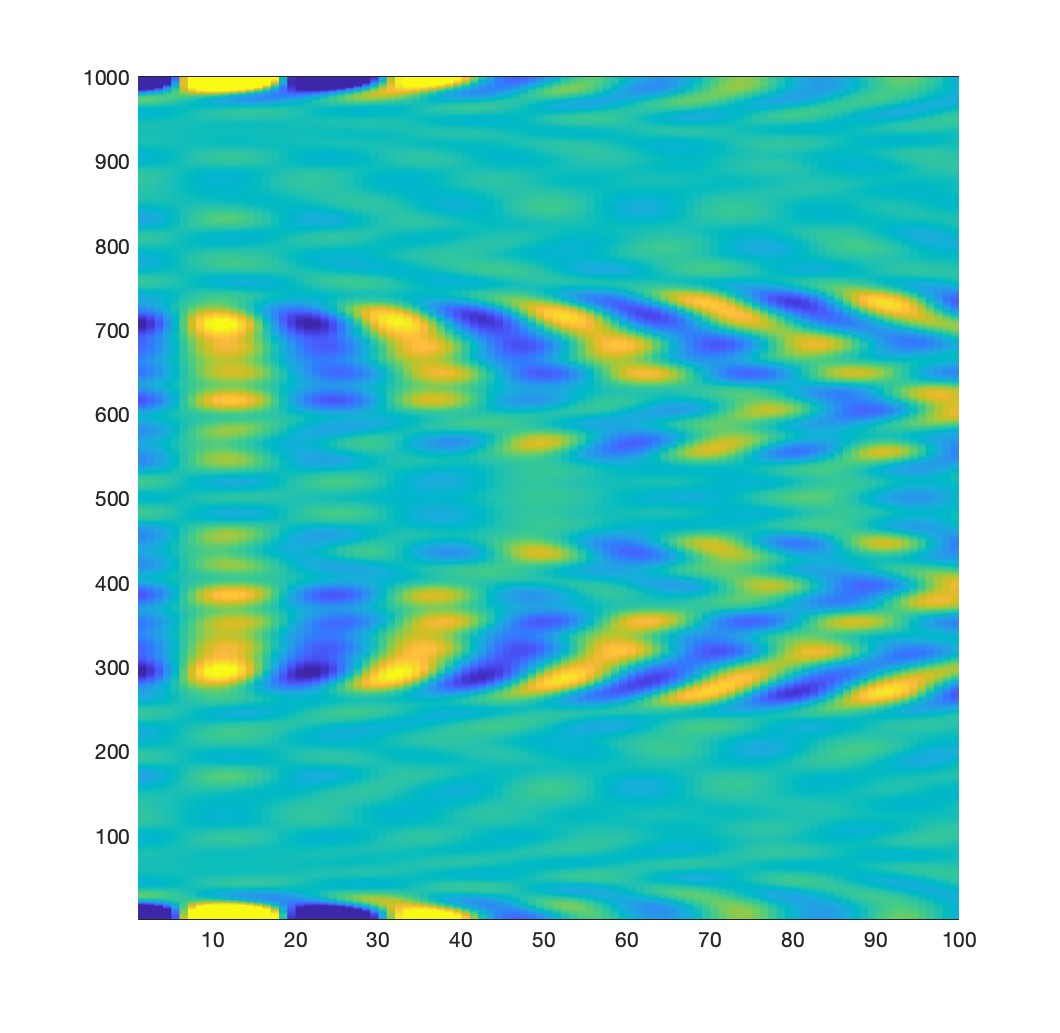
\includegraphics[width=1.0\textwidth]{figures/tmp.jpg}
 \caption{Wave surface from the direct use of the spectra files.}
 \label{tmp}
 \end{center}
 \end{figure}
    
 \begin{figure}
\begin{center}
 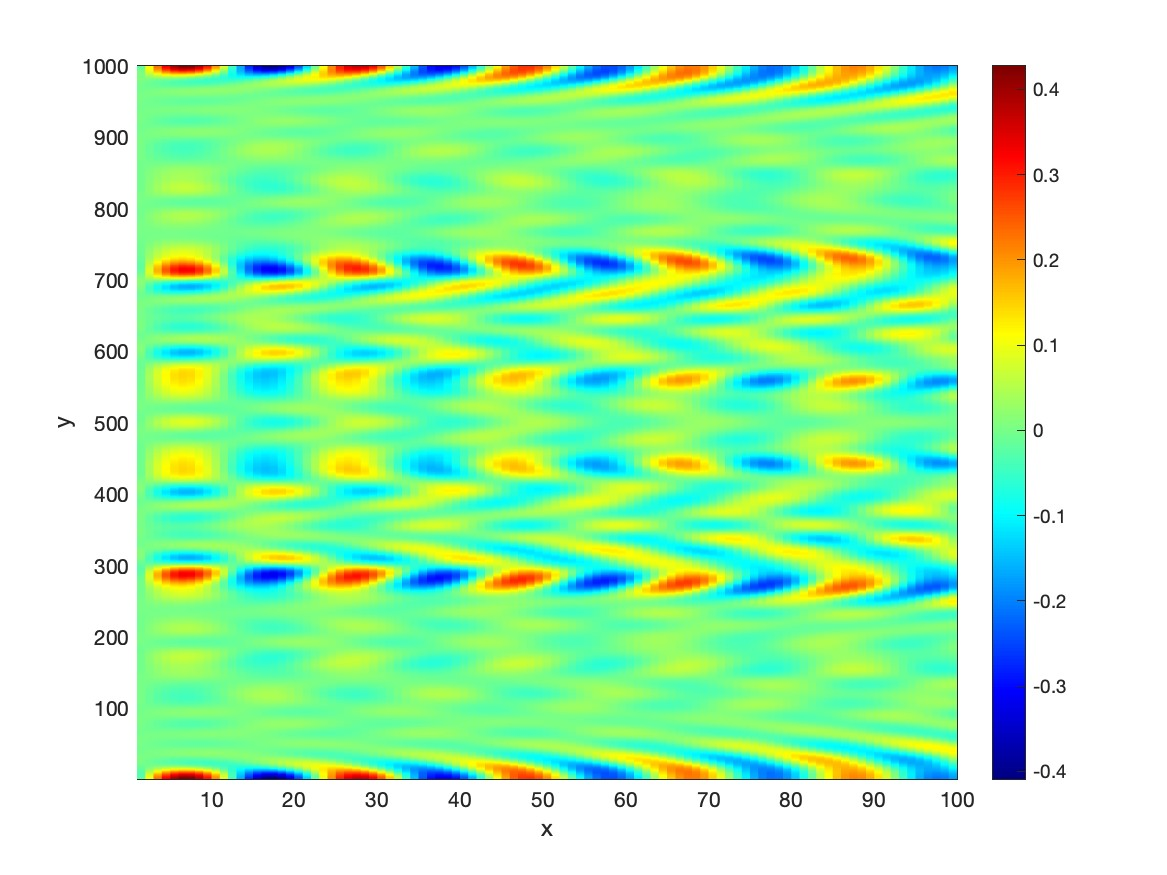
\includegraphics[width=1.0\textwidth]{figures/theory.jpg}
 \caption{Theoretical solution of wave surface based on the given spectra.}
 \label{theoretical}
 \end{center}
 \end{figure}

\section{Time-dependent spectral wavemaker}

The wavemaker was developed based on Larsen and Dancy (1983), Chen et al. (1999), and Zhang et al. (2014) (in /references/ of the package). Waves are generated in a sponge regime, with a damping function of $C_s$. For each wave component, the dependent variables $(\eta, u, v)$ at the grid cell $(i,j)$ are attenuated as
\be
\eta_{i,j} = \eta_{s} + (\eta_{i,j}  - \eta_{s})/C_s
\ee
\be
u_{i,j}  = u_{s} + (u_{i,j}  - u_{s})/C_s
\ee
\be
v_{i,j}  = v_{s} + (v_{i,j}  - v_{s})/C_s
\ee
where $( )_{s}$ is the sources which are  the spatial distribution of any hydrodynamic conditions, such as tidal, surge conditions, and wave conditions. Here, we focus on wave conditions, which are specified based on the linear solution on a flat bottom. The damping function is the   
 same as that used in a sponge layer (see sponge layer section for detail), i.e., at the west boundary,
 \be
 C_s (i,j) = \alpha_s^{\gamma_s^{i-1}}
 \ee
 in which $\alpha_s$ and $\gamma_s$ are parameters. 
 
 The source functions are based on the linear wave solutions at the flat bottom, for component $l$
 \be
 \eta^l = a^l \cos(k_x^l x + k_y^l y - \sigma^l t + \phi^l)
 \ee
 \be
 u^l = a^l \sigma^l \frac{\cosh k^l(h+z_\alpha)}{\sinh k^l h} \cos(k_x^l x + k_y^l y - \sigma^l t + \phi^l))\cos(\theta^l)
 \ee
  \be
 v^l = a^l \sigma^l \frac{\cosh k^l(h+z_\alpha)}{\sinh k^l h} \cos(k_x^l x + k_y^l y - \sigma^l t + \phi^l))\sin(\theta^l)
 \ee
 where $(a, k, \sigma, \theta)^l$ are wave amplitude, wavenumber, angular frequency, and wave angle, respectively, for component $l$. ($k^l_x,k^l_y$) are the wavenumber components in $(x,y)$:  $k^l_x = k^l \cos\theta^l, k^l_y = k^l \sin \theta^l$.  $z_\alpha$ is the $z$ at the reference level defined in the Boussinesq theory.  Note that $\phi^l$ is the phase for component $l$. You will see later that is critical for us to solve the issue. 
 
 The solution for $l=[1,2,... L]$ can be obtained by summating all wave components, for example, for wave surface,
 \be
 \eta = \sum_{l=1}^{L}  a^l \cos(k_x^l x + k_y^l y - \sigma^l t + \phi^l)
 \ee
 To increase the computational efficiency, we separate the time-independent variables from the formula (Shi et al., 2003). For wave component $l$,  we use two-index numbers, $l(l_f, l_d)$, representing indexes for frequency and wave direction, respectively. $l_f = 1 \sim N_f$, $l_d = 1 \sim N_d$, and $L = N_f \times N_d$.
 \be
  \eta = \sum_{l_f}^{N_f} C^{l_f} \cos \sigma^{l_f} t + \sum_{l_f}^{N_f} S^{l_f} \sin \sigma^{l_f} t
  \label{eta}
 \ee
 where
 \be
 C^{l_f} = \sum_{l_d=1}^{N_d} D^{(l_f,l_d)} \cos\left(k_x^{(l_f,l_d)}  x +k_y^{(l_f,l_d)}  y +\phi^{(l_f,l_d)}\right )
 \ee
  \be
 S^{l_f} = \sum_{l_d=1}^{N_d} D^{(l_f,l_d)} \sin\left(k_x^{(l_f,l_d)}  x +k_y^{(l_f,l_d)}  y +\phi^{(l_f,l_d)}\right )
 \ee
 Again, the phase information, $\phi^{(l_f,l_d)}$, is important for solving the issue. (\ref{eta}) provides the linear solution of the wave surface. 
 
 \section{Verification}
 The problem can be verified using a simple matlab program (in package /Linear\_Program/), mk\_spec\_brocc.m. It reads the file, spectra\_data\_1.txt (now brocch\_data.txt), and draws the wave surface based on (\ref{eta}). 
 
 When setting up case1='zero\_phase', $\phi^{(l_f,l_d)} = 0.0$, the wave surface is shown in Figure \ref{zero_phase}. An animation can be found in the folder. You can make an animation by setting TIME=[0:100]. 
 
 When setting up case1='rand\_phase', the program uses the random function $rand$ to generate $\phi^{(l_f,l_d)}$ with random numbers $0 \sim 2\pi$. The solution for the surface is shown in Figure \ref{rand_phase}. 
  \begin{figure}
\begin{center}
 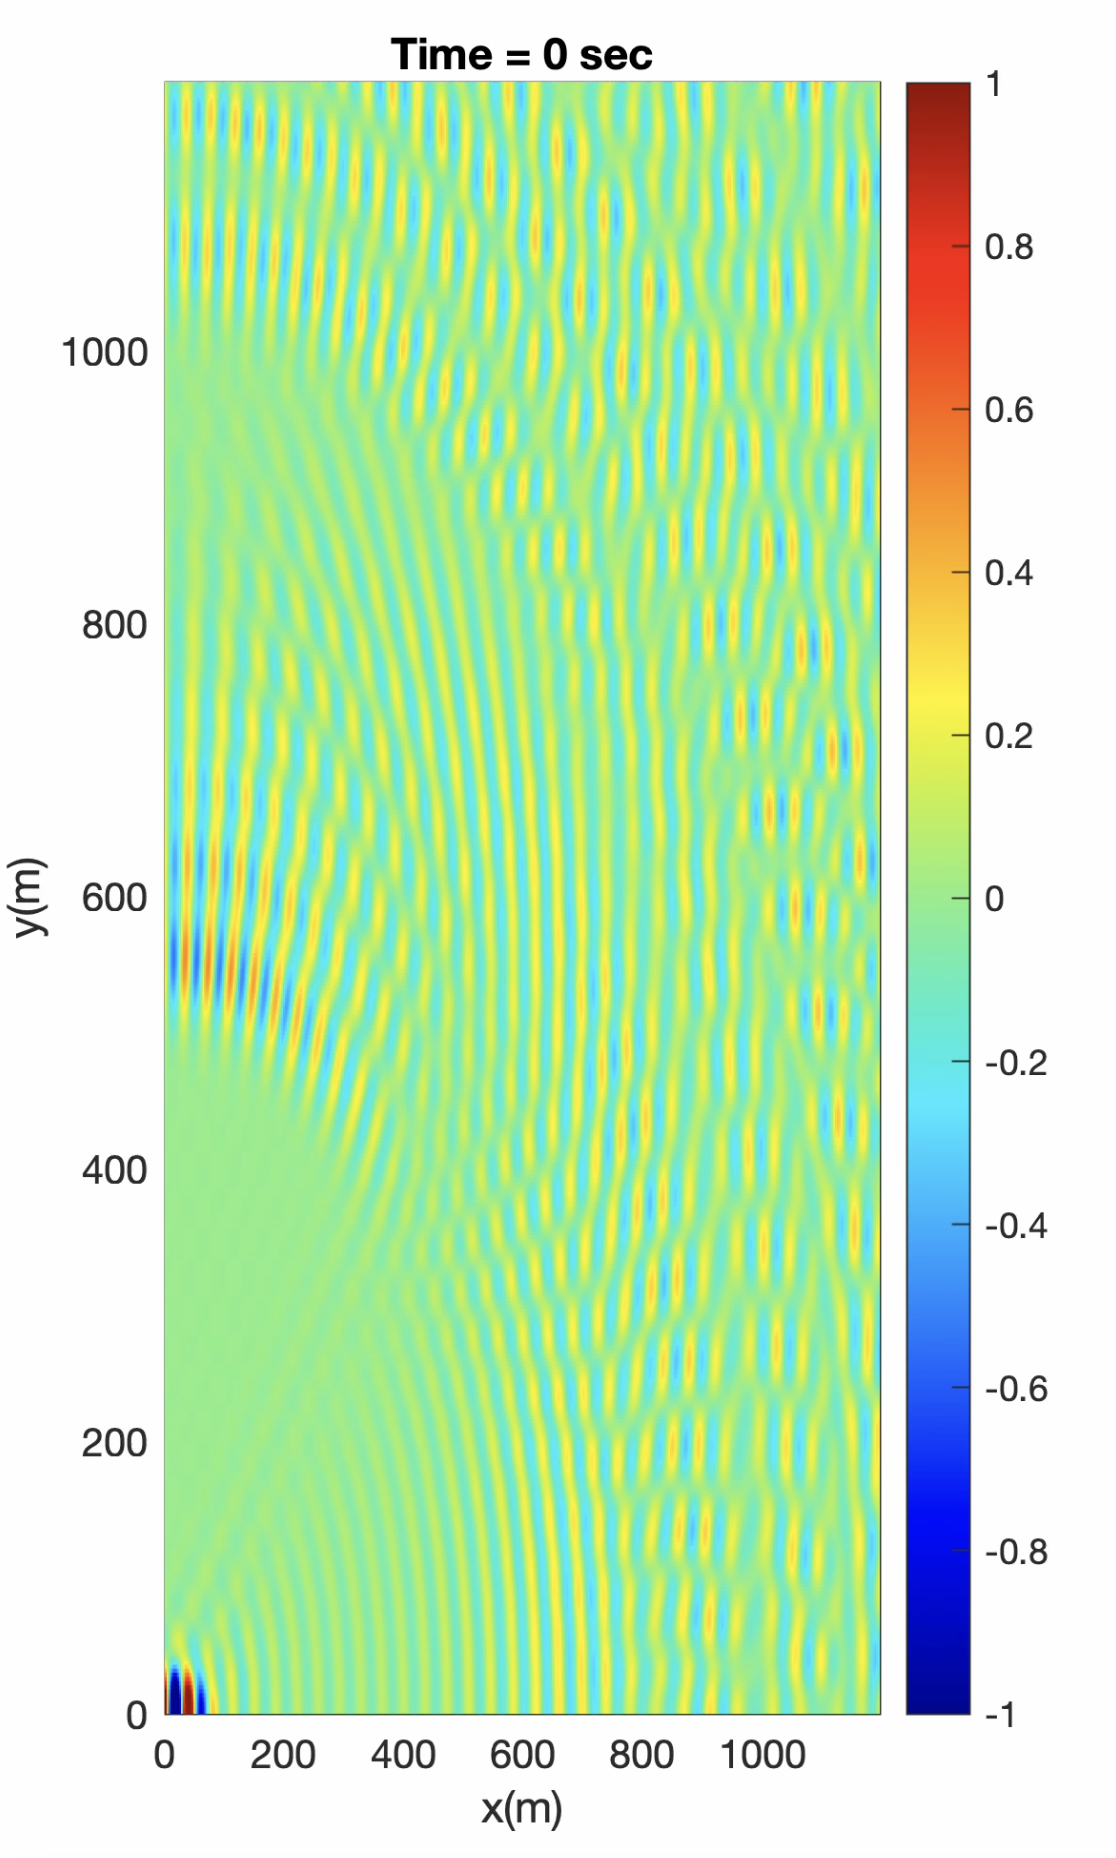
\includegraphics[width=0.6\textwidth]{figures/zero_phase.png}
 \caption{Theoretical solution by setting  $\phi^{(l_f,l_d)} = 0.0$.}
 \label{zero_phase}
 \end{center}
 \end{figure}
  \begin{figure}
\begin{center}
 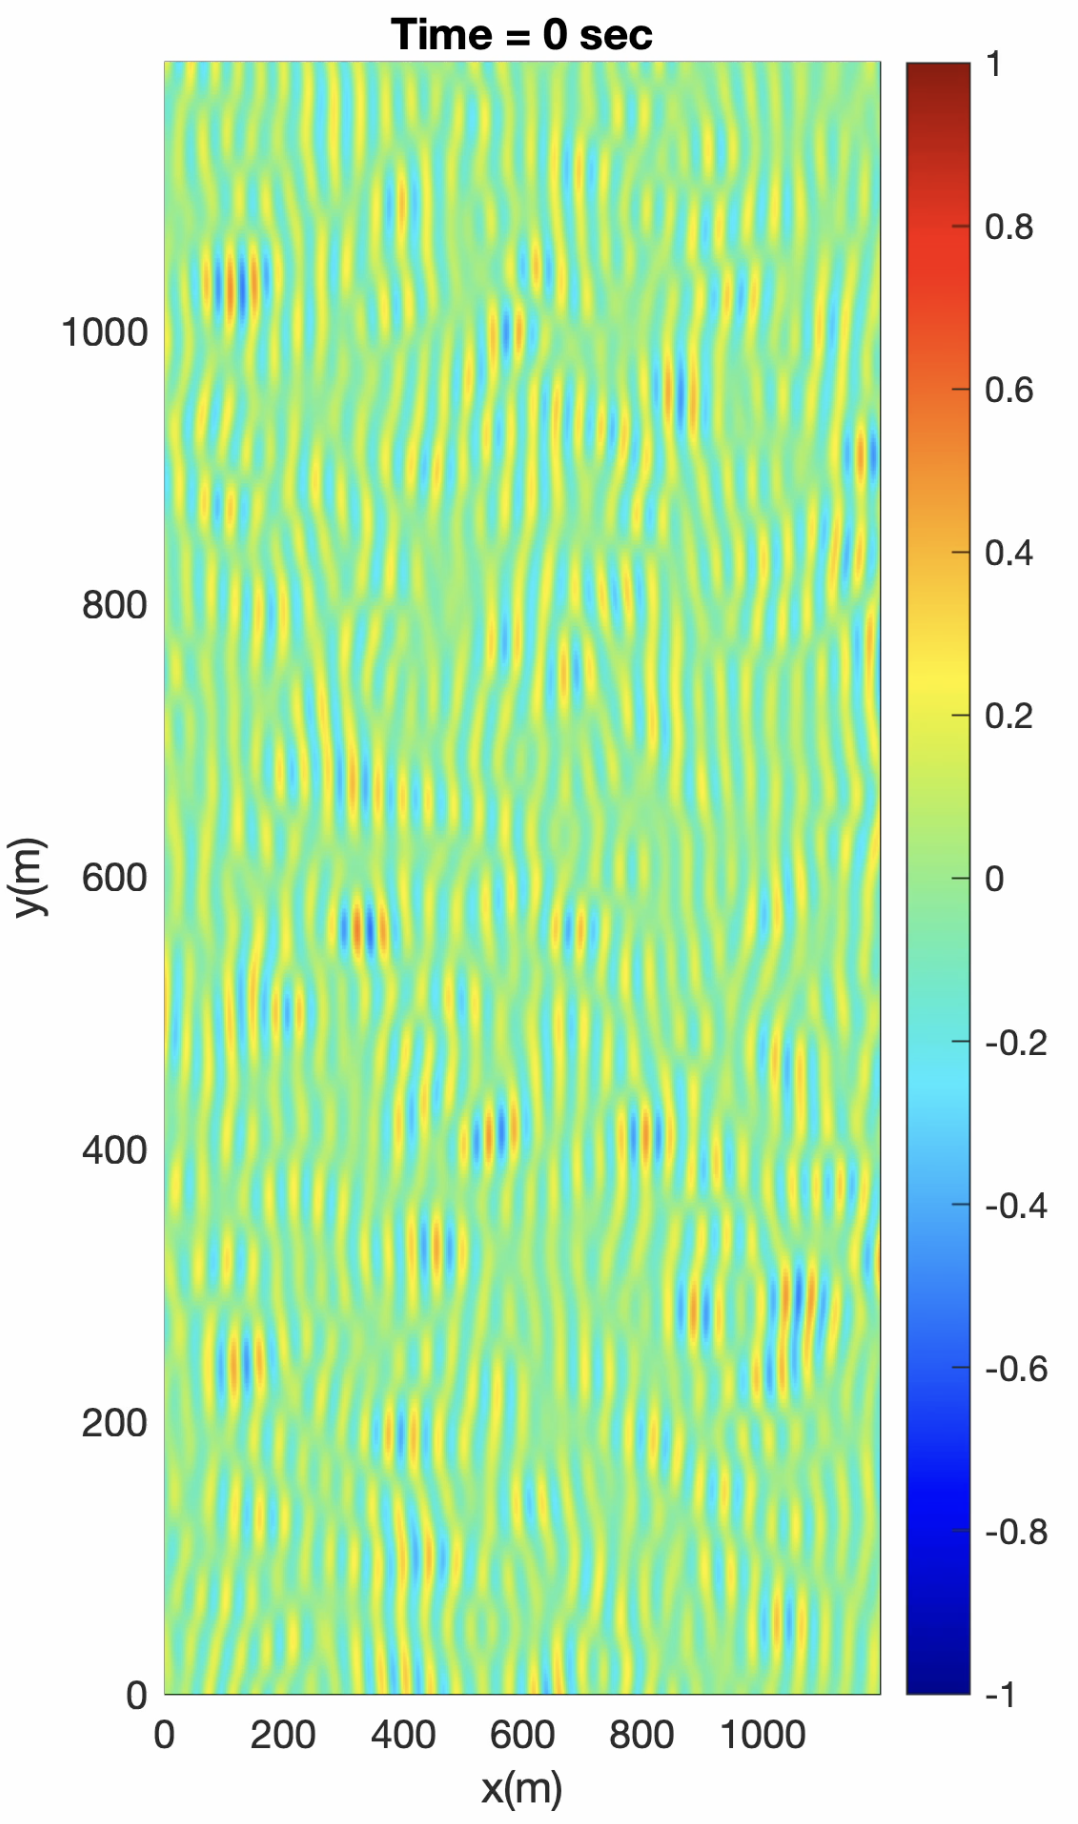
\includegraphics[width=0.6\textwidth]{figures/rand_phase.png}
 \caption{Theoretical solution from random phases.}
 \label{rand_phase}
 \end{center}
 \end{figure}
 
 \section{Code improvement for avoiding the problem}
 The matlab program proved that the issue was caused by the coherence between wave components. Here, the code was modified by adding the random function in the time-dependent spectra module. When a user doesn't provide phase information (a 2D array), the program uses random phases to construct the boundary condition. A check-up output can be made by setting TMP = T in input.txt. The output files for the check-up are a series of surface elevation based on the linear solution (flat bottom), tmp\_xxxxx. A user can compare eta\_xxxxx and tmp\_xxxxx to check consistency. 
 
 As an example, Figure \ref{funwave_theory} shows a comparison between the funwave result (eta\_00150) and the linear solution (tmp\_00150). 
 
 \begin{figure}
\begin{center}
 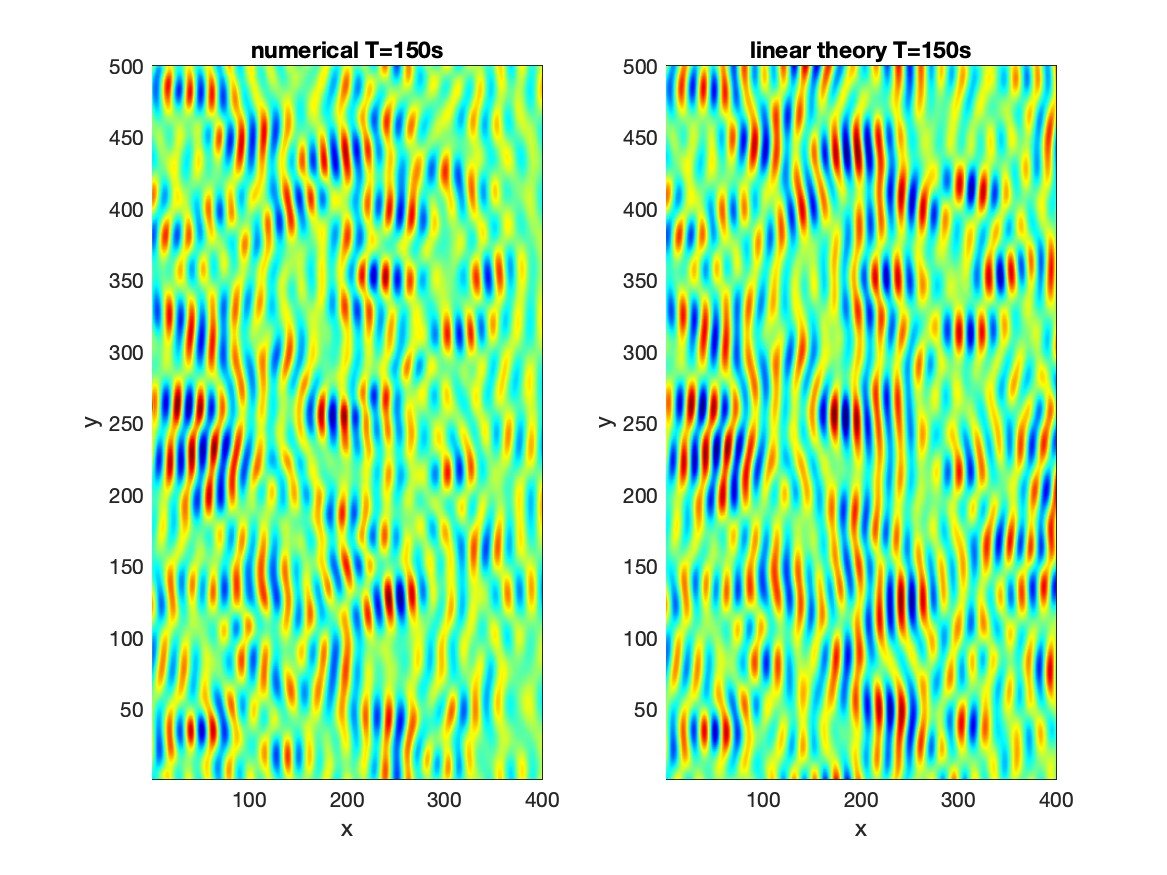
\includegraphics[width=1.0\textwidth]{figures/theory_funwave_150.jpg}
 \caption{Funwave result (left) versus the linear solution (right).}
 \label{funwave_theory}
 \end{center}
 \end{figure}

 \section{Test package}
 
 \href{https://github.com/fengyanshi/TMA_MAKER}{https://github.com/fengyanshi/TMA\_MAKER}
 
 including
 
 1)  \href{https://github.com/fengyanshi/TMA_MAKER/tree/master/LInear_Program}{matlab script}
  
 2)  \href{https://github.com/fengyanshi/TMA_MAKER/tree/master/DOC}{this document}
 
 3)  \href{https://github.com/fengyanshi/TMA_MAKER/tree/master/references}{references}
 
 4)  \href{https://github.com/fengyanshi/TMA_MAKER/tree/master/TEST_CASE}{your case in a smaller domain}

\vspace{1cm}
 
 In conclusion, my feeling is that wave-coherence can be an important problem if the phases are not prescribed in the model. Although setting random phases in the model can't guarantee 0\% wave coherence, it can reduce the coherent patterns. We don't know if wave coherence exists in the open coast without strong coastal geometric feature, as discussed in Zhang et al. (2022).   Salatin et al., (2021) recently addressed the issue in general applications and implemented a new wavemaker in FUNWAVE, which is able to simulate $0 \sim 100\%$ wave coherence. Please refer to the sample cases in the FUNWAVE package /simple\_cases/wave\_coherence/. 
  
  
  
  
\end{document}







